% This paper is copyright 2021 the authors.

% people who might comment on it:
% -------------------------------
% - KSF
% - Kilian Walsh
% - Sanjoy Mahajan
% - David Grier

% to-do items:
% ------------
% - FIX THE FORCE EXPRESSION and discuss it in terms of inner products, tensors, and Einstein summation notation.
% - Put in running head.
% - Overleaf seems to have wrong papersize?
% — Put in the dumbell figure
% - Reconsider the post-equation commas? (HWR SAY).
% — Find references for, and destroy, Bernoulli.
% — Make some comments on the situations in which the ram-pressure force approximation is more appropriate---gale force or lull?

\documentclass{article}
\usepackage[utf8]{inputenc}
\usepackage{graphicx}
\graphicspath{{./}{../ipynb/}}

% math macros
\usepackage{amsmath, amsfonts}
\DeclareMathOperator*{\argmax}{argmax}
\newcommand{\dd}{\mathrm{d}}
\renewcommand{\vec}[1]{\boldsymbol{#1}}
\newcommand{\uvec}{\vec{\hat{e}}}
\newcommand{\tensor}[1]{\mathbb{#1}}
\renewcommand{\flat}{\text{flat}}
\newcommand{\iso}{\text{iso}}
\newcommand{\air}{\text{air}}
\newcommand{\water}{\text{water}}
\newcommand{\boat}{\text{boat}}
\newcommand{\destination}{\text{dest}}
\newcommand{\good}{\text{(good)}}
\newcommand{\better}{\text{(best)}}
\newcommand{\sail}{\text{sail}}
\newcommand{\keel}{\text{keel}}
\newcommand{\hull}{\text{hull}}
\renewcommand{\above}{\text{above}}
\newcommand{\below}{\text{below}}
\newcommand{\vair}{\vec{v}_\air}
\newcommand{\vwater}{\vec{v}_\water}
\newcommand{\vboat}{\vec{v}_\boat}
\newcommand{\vdest}{\vec{v}_\destination}

% text macros
\usepackage{biblatex}
\addbibresource{sailing.bib}
\newcommand{\documentname}{\textsl{Article}}
\newcommand{\secref}[1]{Section~\ref{#1}}
\newcommand{\figref}[1]{Figure~\ref{#1}}

% typesetting adjustments
\makeatletter
\renewcommand\section{\@startsection {section}{1}{\z@}%
  {-3.25ex \@plus -1ex \@minus -.2ex}%
  {1.5ex \@plus .2ex}%
  {\raggedright\normalfont\large\bfseries}}
\makeatother
\setlength{\textwidth}{5.00in}
\setlength{\textheight}{9.00in}
\setlength{\topmargin}{-0.40in}
\pagestyle{myheadings}
\markright{\textsf{Hogg \& Kleban / Ram-pressure model for sailing}}
\newcommand{\captionrule}{\\\rule{\textwidth}{0.2pt}}
\linespread{1.08}
\frenchspacing\sloppy\sloppypar\raggedbottom

\title{\bfseries%
A simple, anisotropic ram-pressure model for sailing}
\author{DWH, MK, others?}
\date{June 2021}
\begin{document}
\maketitle

\begin{abstract}\noindent
    We present a simplified model for the forces on a sailboat.
    Our model is that there is a ram-pressure force on the sail, with a magnitude and direction that depend on the alignment of the relative air--boat velocity with the sail orientation according to an anisotropic drag tensor.
    Similarly, there is a ram-pressure force on the keel, depending on the relative water--boat velocity.
    The resulting expression for the total force on the boat is coordinate-free and consistent with Galilean relativity.
    The solutions corresponding to sailing in steady wind correspond to boat velocities that deliver vanishing total force, given the angles of the sail and keel.
    We use this model to derive simple rules for sailing that are not far off from standard sailing practice, for sailing in different directions (including upwind).
    One consequence of this model is that a sailboat does not move (relative to the water) precisely in the direction that its keel points (the direction of the prow); it moves slightly downwind of that.
    Another consequence is that it is possible for an extremely anisotropic (extremely well designed) boat to sail downwind (relative to the water) \emph{faster than the wind}, on a tacking course.
    Interestingly, nothing about the mechanical model or discussion depend on the \emph{curvature} of the sail, in contradiction to some folk explanations of sailing.
\end{abstract}

\section{Introduction}\label{sec:intro}

KLEBAN: Write things about ddwfttw, maybe?

HOGG: Stuff about Bernoulli and flying and aerofoils that turned out to be wrong; a motivation to reconsider sailing too.

\section{Ram-pressure sailboat}\label{sec:boat}

We are going to work in 2D, with velocities $\vec{v}$ and forces $\vec{F}$ that are column vectors (or $2\times 1$ matrices).
To stay coordinate-free, we are going to talk about angles as orientations of unit vectors like $\uvec_{\perp\sail}$ and $\uvec_{\parallel\sail}$ (which will be defined below).
If you prefer to think in terms of angles, you can choose a coordinate system and then
\begin{align}
    \uvec_{\perp\sail} &= \begin{bmatrix}\cos\theta_\sail \\ \sin\theta_\sail\end{bmatrix} ~ ; ~ \uvec_{\parallel\sail} = \begin{bmatrix}-\sin\theta_\sail \\ \cos\theta_\sail\end{bmatrix} ~,
\end{align}
for some angle $\theta_\sail$ in that coordinate system.
We won't particularly use angles much in what follows, but if you want to come back to angles, you can take the arctangent of the components of $\uvec_{\perp\sail}$.

Our sailboat is going to be a simple anisotropic object such that wind that hits its planar sail produces a ram-pressure force perpendicular to the surface of the sail,
and water that hits its planar keel produces a ram-pressure force perpendicular to the surface of the keel.
We can construct the complete force law on the sailboat by thinking about ram-pressure forces on surfaces.
If the fluid (air or water in this case) is thought of as being composed of particles that bounce elastically off of a flat surface of area $A$, then the ram-pressure force on that surface is
\begin{align}\label{eq:flat}
    \vec{F}_\flat &= \eta\,\rho\,A\,(\uvec_\perp^\top\vec{v})^2\,\uvec_\perp ~,
\end{align}
where $\eta$ is a dimensionless prefactor, $\rho$ is the density of the fluid, $\uvec_\perp$ is the unit vector perpendicular to the surface (oriented such that it points down-flow), $\vec{v}$ is the velocity of the fluid in the rest frame of the surface, and $\uvec_\perp^\top\vec{v}$ is the scalar inner product (dot product) of the two vectors.
Na\"ively in the particle-collision model the prefactor $\eta$ is 2, but in the world of real fluids it depends on the shape of the surface, the velocity, and (if things are tiny) the viscosity\footnote{%
Viscosities only matter for very small objects, much smaller than sailboats. The way to see this is HOGG (CITE).}.
We're going to treat $\eta$ as an uninteresting constant; in particular we are going to assume that it doesn't depend on velocity, such that it can be combined with the area $A$ in everything that follows.
If you like thinking about tensors, the flat-surface force \eqref{eq:flat}  can be thought of as a tensor expression, in which $\rho$, $A$, and the unit vectors are combined into a three-index (order-three) tensor $\tensor{A}$, which is then contracted onto the velocity twice:
\begin{align}
    \tensor{A} &\equiv \eta\,A\,\uvec_\perp\,\uvec_\perp^\top\otimes\uvec_\perp^\top ~.
\end{align}
In Einstein summation notation, the three-index tensor is contracted as follows
\begin{align}
    [\vec{F}_\flat]_i &= \rho\,[\tensor{A}]_{ijk}\,[\vec{v}]_j\,[\vec{v}]_k ~,
    \\
    [\tensor{A}]_{ijk} &= \eta\,A\,[\uvec_\perp]_i\,[\uvec_\perp]_j\,[\uvec_\perp]_k
    ~,
\end{align}
where the $[\vec{v}]_i$ notation indicates the $i$th component or coordinate of the vector, the tensor $\tensor{A}$ has three indices, and the repeated indices are summed over.
If, instead of a planar object, you have an isotropic object (a sphere in fully 3D situations, an axi-symmetric boat in our 2D water world), the ram-pressure force becomes
\begin{align}\label{eq:iso}
    \vec{F}_\iso &= \eta\,\rho\,A\,|\vec{v}|\,\vec{v}
\end{align}
where $\eta$ is a (different) dimensionless prefactor, $A$ is now the cross-sectional or projected area of the surface, and $\vec{v}$ is still the fluid velocity in the rest frame of the object.
Again $\eta$ depends on velocity, but again we are going to ignore that.

Our model for a sailboat is going to be that it is a composite object, composed of a flat sail, a flat keel, and an isotropic partially submerged hull.
Thus the ram-pressure force on the sailboat will have four components, a force on the flat sail from the air, a force on the flat keel from the water, a force on the hull from the air, and a force on the hull from the water.
This model is extremely simplistic!
In some sense it is the closest possible model to the spherical cow that will sail non-trivially.
In detail the forces from the air are given by
\begin{align}
  \vec{F}_\air &= \vec{F}_{\sail-\air} + \vec{F}_{\hull-\air}
  \\
  \vec{\Delta v}_\air &\equiv \vair - \vboat
  \\
  \vec{F}_{\sail-\air} & = \rho_\air\,A_\sail\,(\uvec_{\perp\sail}^\top\,\vec{\Delta v}_\air)^2\,\uvec_{\perp\sail}
  \\
  \vec{F}_{\hull-\air} & = \rho_\air\,A_{\above}\,|\vec{\Delta v}_\air|\,\vec{\Delta v}_\air ~,
\end{align}
where we have dropped the $\eta$ prefactors (or really combined them with the area constants), $\vair,\vboat$ are the velocities of the air and boat, $A_\sail$ is an area related to the area of the sail, $\uvec_{\perp\sail}$ is a unit vector perpendicular to the plane of the planar sail, and $A_{\above}$ is an area related to the area of the boat's hull that is above the water surface.
Similarly, the forces from the water are given by
\begin{align}
  \vec{F}_\water &= \vec{F}_{\keel-\water} + \vec{F}_{\hull-\water}
  \\
  \vec{\Delta v}_\water &\equiv \vwater - \vboat
  \\
  \vec{F}_{\keel-\water} & = \rho_\water\,A_\keel\,(\uvec_{\perp\keel}^\top\,\vec{\Delta v}_\water)^2\,\uvec_{\perp\keel}
  \\
  \vec{F}_{\hull-\water} & = \rho_\water\,A_{\below}\,|\vec{\Delta v}_\water|\,\vec{\Delta v}_\water ~,
\end{align}
where the sail is replaced by the keel everywhere, and $A_{\below}$ is an area related to the area of the hull below the water surface.
HOGG NEED WE SAY MORE ABOUT THESE? PROBABLY YES THERE ARE COMMENTS TO BE MADE.

\section{Steady sailing}\label{sec:steady}

Mathematically, steady sailing (constant $\vboat$) in steady wind and steady current (constant $\vair, \vwater$) is given by
\begin{align}\label{eq:sailing}
    \vec{F} &= \vec{F}_\air + \vec{F}_\water = \vec{0} ~.
\end{align}
If we want to operationalize steady sailing in code, steady sailing can be thought of as a root-finding problem, in which we find the vector $\vboat$ that makes \eqref{eq:sailing} true, given the orientations $\uvec_{\perp\sail}, \uvec_{\perp\keel}$ of the sail and keel.
This is a root-finding problem that (probably) has no closed form\footnote{%
It might be interesting to note that the flat-surface force \eqref{eq:flat} is a vector-valued quadratic form, so if one constructed the sailboat model completely from flat surfaces, the force law, in this approximation would be a quadratic form.
That might lead to a closed-form solution for the equation \eqref{eq:sailing} of steady sailing.}.
We solve equation~\eqref{eq:sailing} numerically in the code associated with this \documentname\footnote{%
HOGG GIVE LINK HERE}
by means of the vector generalization of Newton's method (we return to this in \secref{sec:implementation}).

HOGG: Define direction cosines with the wind, and with boat parts, using vectors. ADD THOSE direction cosines to the figure panels.

In \figref{fig:steady} we show examples of steady sailing, for a wide range of orientations of the keel and sail.
All these examples are shown in the water rest frame.
The boat has four free parameters $(A_\sail,A_\keel,A_{\above},A_{\below})$ all with units of area (or really three independent dimensionless ratios of these four areas).
The values we chose for these four parameters are given in \secref{sec:design} and discussed in detail there.
\begin{figure}[t!]
  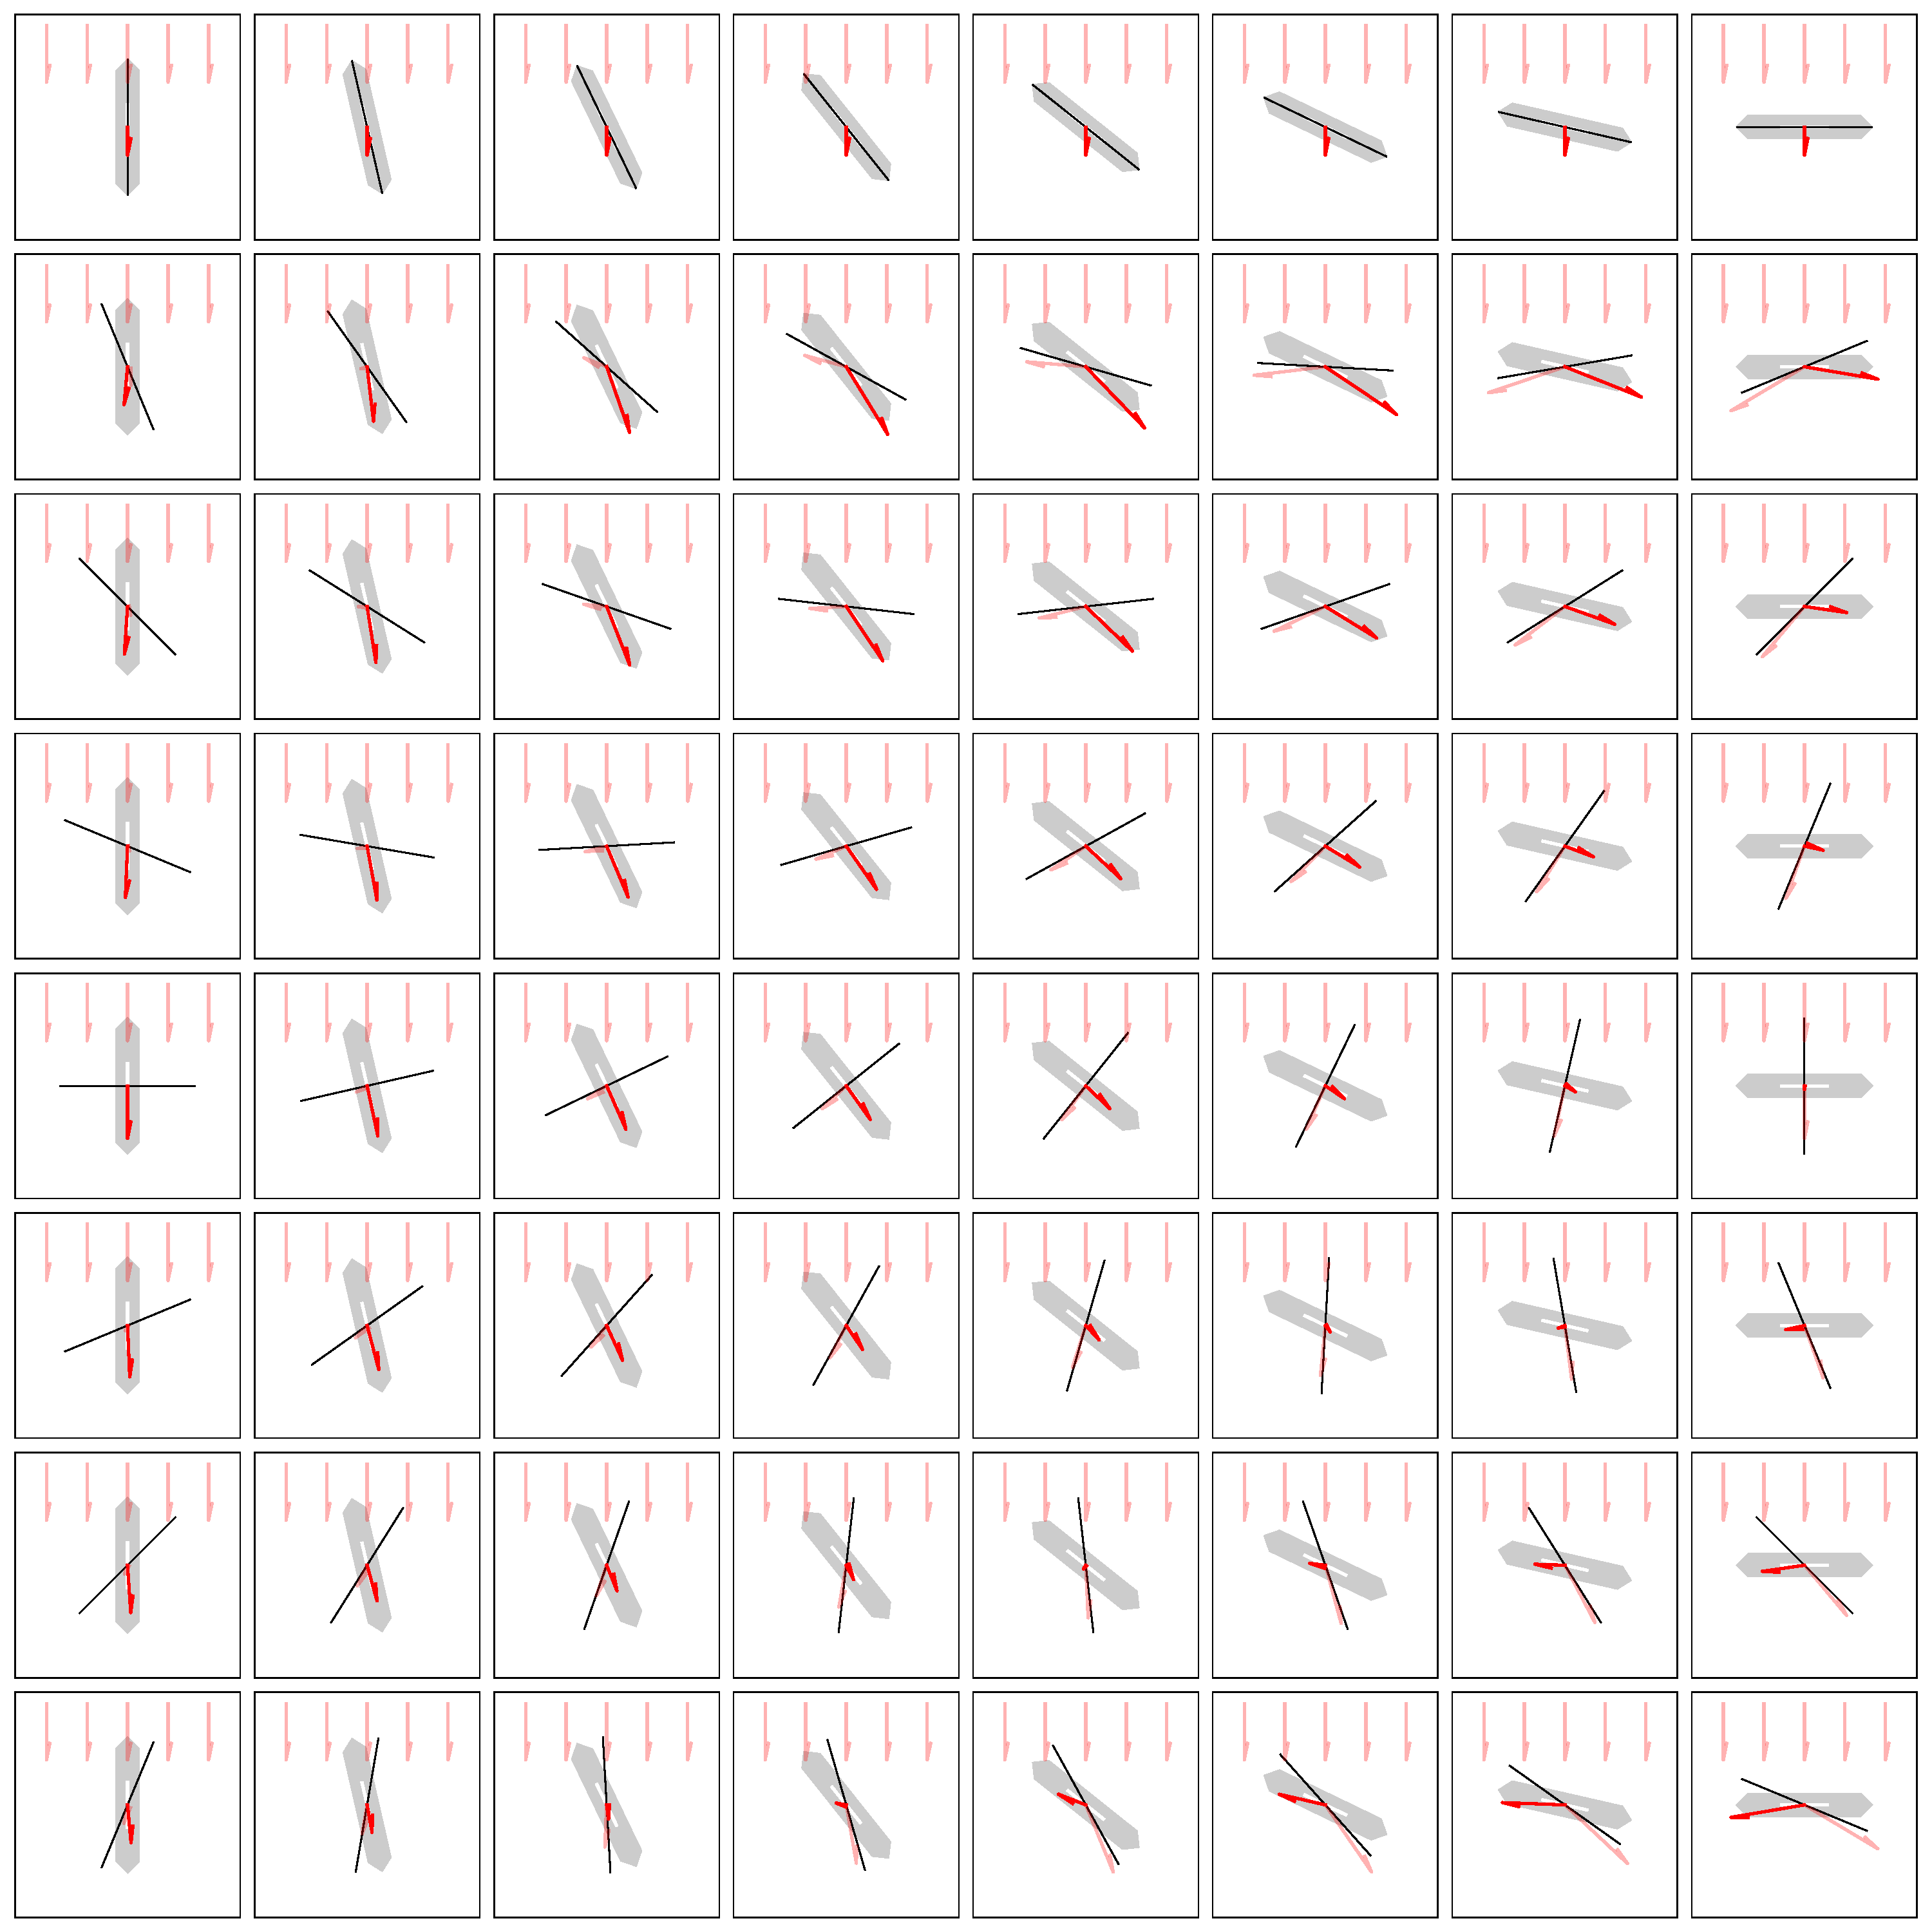
\includegraphics[width=\textwidth]{steady.pdf}
  \caption{Visualizations of the boat velocity $\vboat$ for different settings of the orientations of the keel and sail, all presented in the water rest frame.
    The views are top-down; the keel is represented by a thick grey line, the sail is represented by a thin black line, and the wind and boat velocities are represented by black arrows.
    Most of the settings of the keel and sail lead to downwind travel, but a few lead to upwind travel, for example XXX and YYY. HOGG LABEL THE PANELS.\label{fig:steady}\captionrule}
\end{figure}

In \figref{fig:hourglass} we show the distribution of boat velocities one obtains if one randomly orients one's sail and keel....HOGG
HOGG: Put the random-dot hourglass figure here.

HOGG: Comments: You can see from the figures that you don't sail DIRECTLY in the direction the keel is pointed.

HOGG: Right now, the concept of forwards and backwards is a bit soft; our boat is quadrupolar! But we will get more serious about deliberately sailing in the correct direction in the next Section.

HOGG: Comment: You can't achieve zero velocity wrt either the air or the water.

HOGG: Comment: It is easy to sail downwind fttw.

HOGG: Comment: It is easy to sail faster than the wind speed.

HOGG: Comment: It is easy to sail upwind. If the boat is AMAZING you can sail upwind faster than the wind! Probably not possible in practice? KLEBAN?

HOGG: Comment: You can't sail directly into the wind, or within XXX radians of directly into the wind. This XXX depends on dimensionless sail and boat ratios.

\section{Good sailing}\label{sec:good}

In \secref{sec:boat} we showed how the boat moves, given any arbitrary setting of the orientation of the keel and the sail.
However, one doesn't sail by randomly setting the keel and sail!
One sails by pointing the boat in some direction and then setting the sail (or sails) appropriately.
In our simple, ram-pressure boat, how should we set the planar sail?

HOGG: IN THIS SECTION EXPLICITLY DEFINE ``GOOD SAILING''.
\begin{align}\label{eq:good}
    \uvec_{\perp\sail}^\good &\leftarrow \argmax_{\uvec_{\perp\sail}} \left[\uvec_{\parallel\keel}^\top\,(\vboat-\vwater)\right] ~,
\end{align}
where .... HOGG IMPLICITLY $\vboat-\vwater$ is a function of all the properties of the world and the boat boat, along with the orientation of its keel and sail.

HOGG: FIGURE showing good sailing for a set of boat orientations.

HOGG: Figure showing direction cosines of sail relative to keel/boat orientation.

HOGG: Put the equivalent of the hourglass figure.

HOGG: Comment: The settings of the sail look ``tight'' relative to standard sailing practice. But this boat has flat sails, so it's hard to compare the exact settings with sailor experiences (which are all with curved sails).

HOGG: Final comment: But this is not the BEST a sailor can do...

\section{Better sailing}\label{sec:better}

HOGG IN THIS SECTION EXPLICITLY DEFINE ``BETTER SAILING''.

A type-A sailor---or maybe a competetive sailor---is trying to get from a current position to a destination as quickly as possible\footnote{%
We don't particularly endorse this attitude towards sailing. The journey \emph{is} the destination.}.
Our view is that this sailor should start by specifying the unit vector $\uvec_\destination$ that points from the current position of the boat towards the destination of the boat.
The sailor should then maximize the scalar product $\uvec_\destination^\top\,\vboat$
\begin{align}\label{eq:better}
    \uvec_{\perp\sail}^\better,\uvec_{\perp\keel}^\better &\leftarrow \argmax_{\uvec_{\perp\sail},\uvec_{\perp\keel}} \left[\uvec_\destination^\top\,(\vboat-\vdest)\right] ~,
\end{align}
where $\uvec_{\perp\sail}^\better,\uvec_{\perp\keel}^\better$ are the best settings of the orientations of the keel and sail, given the direction $\uvec_\destination$ to the destination, and (because we are Galilean-relativistic) this velocity is relative to the velocity $\vdest$ of the destination (which might not be stationary with respect to the water).
In this expresion \eqref{eq:better}, implicitly $\vboat$ is being thought of as a function of these orientations (and more).
Note that the sailor \emph{does not necessarily want} to travel directly towards the destination:
The sailor wants to make as much progress as possible in that direction, but is willing to tack back-and-forth to get there, if it gets the boat there faster.
So the metric really is the projection of the boat velocity onto the displacement vector pointing from the current position of the boat to the destination.

While this is simple to state, the numerical optimization hurts...HOGG

HOGG PUT FIGURES HERE SHOWING THE OPTIMAL SETTINGS OF SAIL AND KEEL ORIENTATIONS FOR DIFFERENT DESTINATION DIRECTIONS.

Now if you want to plan a complete path or journey for the sailboat in (unrealistically) steady wind, you... HOGG

HOGG PUT FIGURES HERE SHOWING TRAJECTORIES FOR SIMPLE JOURNEYS. MAYBE??

\section{Boat properties and boat design}\label{sec:design}

HOGG: In the above experiments and diagrams we made use of a boat with the following properties....

HOGG: These properties might seem unreasonable! However, remember that our boat is just a brutal approximation.
A true boat has sails that are globally curved\footnote{%
In the local-curvature or Riemann-curvature senses, sails are not (very) curved; after all, they are made from flat pieces of fabric.
However, they are curved in the global or colloquial sense: Different patches of the sail have differently oriented normal vectors.},
and forces that are different from these pure ram-pressure forces.
The curvature of the sails will in general rotate the air force vectors towards the direction in which the boat is pointed.

HOGG show how the hourglass plots depend on the qualities of the boat, such as: Relative area of sail and keel. Relative area of hull and keel. Etc.

\section{Numerical implementation notes}\label{sec:implementation}

HOGG: Newton's method (CITE), invert, solve, etc.
Note that in practice, Newton's method works amazingly well.
For Newton's method we make use of the derivatives---HOGG GIVE HERE THE DERIVATIVES of the ram-pressure expressions---which are order-2 tensors.

HOGG: How we implement GoodSailing(tm) and BetterSailing(tm). It's a mess!

\section{Discussion}\label{sec:discussion}

HOGG: What did we find? What's important about that?

HOGG: Galilean symmetry, coordinate freedom?

HOGG: What were our assumptions? What are the myriad ways in which those assumptions must be wrong? For example, boat has an asymmetry in the wind too, so really the boat must also matter. Viscosity; why can we ignore it? But turbulence; we can't ignore that! Constant $\eta$ is also wrong.

HOGG: Take some time to bash the Bernoulli bullshit.

HOGG: Even BetterSailing(tm) is not the best you can do, because you have to do complete successful path planning, and coming about costs time. So you will sail beyond the limits of BetterSailing(tm) if you do this correctly. This is out of scope for this \documentname.

HOGG: All code used to make the figures in this \documentname{} are available HOGG WHERE?

\paragraph{Acknowledgements:}
It is a pleasure to thank Hans-Walter Rix (MPIA) for valuable discussions.

\raggedright
\printbibliography
\end{document}
